\documentclass[11pt]{article}
\usepackage{coling2016}
\usepackage{times}
\usepackage{url}
\usepackage{latexsym}
\usepackage{hyperref}
\usepackage{color}
\usepackage{amsmath}
\usepackage{epsfig}
\usepackage{graphicx}
\newcommand{\figref}[1]{Figure \ref{#1}}
\newcommand{\tabref}[1]{Table \ref{#1}}
\usepackage{epstopdf}
\usepackage{booktabs}
\usepackage{diagbox}
\usepackage{array}
%\usepackage{float}
\usepackage{stfloats}
\usepackage{multicol}
\usepackage{multirow}
\usepackage{threeparttable}
\usepackage[multiple]{footmisc}

\usepackage[english]{babel}

%\usepackage[skip=2pt,font=scriptsize]{caption}
\newcolumntype{I}{!{\vrule width 1pt}}
\newlength\savedwidth
\newcommand\whline{\noalign{\global\savedwidth\arrayrulewidth
                            \global\arrayrulewidth 1pt}%
                   \hline
                   \noalign{\global\arrayrulewidth\savedwidth}}
\newlength{\Oldarrayrulewidth}
\newcommand{\Cline}[2]{%
  \noalign{\global\setlength{\Oldarrayrulewidth}{\arrayrulewidth}}%
  \noalign{\global\setlength{\arrayrulewidth}{#1}}\cline{#2}%
  \noalign{\global\setlength{\arrayrulewidth}{\Oldarrayrulewidth}}}

\newcommand{\KZ}[1]{\textcolor{blue}{Kenny: #1}}
\newcommand{\BF}[1]{\textcolor{red}{Bean: #1}}
\newcommand{\TJ}[1]{\textcolor{red}{Jia: #1}}
\newcommand{\YZ}[1]{\textcolor{red}{Yizhong: #1}}
\newcommand{\cut}[1]{}

\title{Towards Non-projective High-Order Dependency Parser}
\author{Wenjing Fang  \and Kenny Q. Zhu  \and Yizhong Wang \and Jia Tan\\
  Shanghai Jiao Tong University \\
  {\tt \{littlebeanfang,kzhu\}@sjtu.edu.cn} \and {\tt \{eastonwyz,tjtanjia.tan\}@gmail.com}\\
  }
%\date{}
\begin{document}
\maketitle
\begin{abstract}
  %Existing data-driven dependency parsers mainly fall into two classes:
%graph-based and transition-based. However, both methods draw some distinctions
%from the way that we human beings perform the parsing task.
This paper demonstrates a novel high-order dependency parsing framework that
targets non-projective languages.\blfootnote{This work is licensed under a Creative Commons Attribution 4.0 International License. License details: http://creativecommons.org/licenses/by/4.0/}
It imitates how a human parses sentences in an intuitive way.
At every step of the parse, it determines which word is the easiest to
process among all the remaining words, identifies its head word and then
folds it under the head word.
This greedy framework achieves competitive accuracy on WSJ evaluation set
and shows additional advantage on the non-projective corpus.
%\BF{multi-lingual}
 % \BF{redo experiment,not the accurate number}
Further, this work is flexible enough to be augmented with other
parsing techniques.~\footnote{Kenny Q. Zhu is the corresponding author
and is partially supported by NSFC Grant No. 61373031.}
\end{abstract}

\section{Introduction}

Protein$-$protein interactions (PPIs) are of central importance for the majority of biological functions, such as signal transduction, metabolic pathways, molecular dynamics, and protein networks\cite{Hoffmann.Krallinger.ea:2005}, for they serve as the most fundamental building blocks of the entire interacademic systems of any organisms. Collecting data on pairwise interaction relationships is essential for multiple purpose, including identification of modules with certain functionality\cite{Spirin.Mirny.03}, mapping diseases to dominated genes\cite{Ideker.Sharan.08}, and after all, understanding wholistic metabolic/genetic networks from a system biology perspective.

A lot of databases have been built to store protein and genetic interactions from major model organism species and are available in various standardized formats, such as MINT\cite{Zanzoni.Montecchi-Palazzi.ea:2002}, BIND\cite{Bader.ea:2003}, BIOGRID\cite{DBLP:journals/nar/StarkBRBBT06}, etc. Among those mainstream databases, the data largely rely on voluntary reports by scientists or researchers, besides, comprehensive curation efforts become indispensable for the sake of accuracy. However, the amount of biology-related literatures with respect to protein interactions grows explosively and thus make it either impossible or impractical to manually detect PPI information anymore.

Considering huge amount of PPI information with great wealth hidden in published papers, in recent years, numerous mining techniques have been proposed that aim to extract PPI information automatically from free text, especially machine learning, information retrieval, and natural language processing\cite{DBLP:journals/bib/WinnenburgWPDS08}.These approaches can be roughly categorized into three classes: co$-$occurrence, rule$-$based, and machine learning. 

Co$-$occurrence is the approach with most simplicity and naivete. Just as its name implies, this method intends to find out pairs of proteins that co-occur in the same context. The scope of "same context" ranges from phrase, sentence, paragraph to whole abstract, even document. The underlying assumption is that whenever two proteins are mentioned together by authors, chances are high that there is some kind of relationship between them. However, however, in-context closeness even semantic relation does not necessarily represent actual biological interaction. As a consequence, a large fraction of candidate pairs are mismatched inevitably, causing a high recall but low precision.

The second approach is rule-based extraction, in other words, pattern matching. There are many types of rules, most of them concern natural language processing (NLP). One way is to specify hand-crafted regular expressions before hand, which mostly lean on language usage preference. Besides, by using full or partial (shallow) parsing strategies, more information would be acquired, such as part-of-speech taggers, local dependencies between syntactic components, context-free grammar\cite{DBLP:journals/bioinformatics/TemkinG03}, and full sentence structure. Compared to co$-$occurrence, rule-based approach enjoy better precision but much lower recall. In addition, since the rules are usually derived from training data, that is to say, the improper choice of training data would be significantly lethal, therefore quality of extraction is invariably instable and may not applicable to other data.

The third and most commonly used approach use machine learning techniques, in this case, the task to extract protein$-$protein interactions turns out to be a binary classification problem. Each protein pairs are represented along with a set of features, which is associated with their context, then a well$-$defined classifier gives the answer whether the candidate protein pairs is classified to be qualified PPI. (TO BE FURTHER FILLED!!!)

In this paper, we introduce a general bootstrapping framework for Protein$-$protein interaction extraction from natural text.Our method differs from most of the previous works in three aspects:

(1)The extraction process is driven by only tiny fraction of training data, which are regarded as seed data. In each round, it would derive reliable patterns automatically from seed data, then extract more positive PPI pairs consequently, what's more, the seed data would be augmented by the newly extracted results with high confidence.

(2)multiple graph kernel. 

(3)various evaluation.




\section{Framework}
%\BF{workflow figure to show the framework}
%\begin{multicols}{2}
%\begin{figure*}
%\centering
%\includegraphics[width=2\columnwidth]{sysoverviewgrapheps.eps}
%\caption{Framework wrokflow} \label{fig:workflow}
%\end{figure*}
%\end{multicols}
%\KZ{In the framework, say ``Output Parse'' instead of ``Output File.''}
The general architecture of the our parser is shown in \figref{fig:workflow}
and is divided into training phase and parsing phase.
%We take training treebank as input, which carries the
%essential information (we only use FORM and POSTAG) and
%gold dependency parses.

\begin{figure}[th]
\centering
\epsfig{file=sysoverviewgrapheps.eps, width=\columnwidth}
\caption{Sequence Based Parser Framework}
\label{fig:workflow}
\end{figure}

{\bf Training:} The preprocessing step generates oracle sequences
from the gold standard parse trees. Only the word forms and the POS tags 
in these parse trees are used. Here, we assume that a child node is
easier to process than its parent node and it is supposed to be attached
before its parent. \footnote{By this rule, multiple gold sequences
can be generated from one dependency tree. In this paper, when a parent node
has multiple children, we generate the sequence by a left-to-right order.}
%\KZ{Which one do we use or do we use all of them?}
%\footnote{
%For example, a bottom-up, breadth-first traversal of the gold parse tree or oracle transition
%process order from Malt Parser are both gold sequences.}
%and further discussion is deferred to Section 4.
%\TJ{maybe they will ask which one is the best; needs some explanations here}
We then train respectively a graph-based head mapper (a.k.a. decoder)
from the gold sequences and the gold parses, and a sequence predictor
from the gold sequences.

{\bf Parsing:} Given an input sentence, the sequence predictor
outputs a feasible decoding sequence, which is a permutation of
the words in the input. For each word in this sequence,
the head mapper returns its best head word according to a scoring function
while employing a cycle detection mechanism.
The process continues until all words in the sentence have found their
heads.
%(except manually introduce ROOT node in dependency parsing).
%For a sentence with $N$ words, the final result consists of ($N+1$) nodes
%and constructed $N$ arcs.
The procedure guarantees to produce a tree structure eventually.
\cut{
We implemented a simple version of this framework,
%and released the source code as well as the evaluation data\footnote{\urlstyle{same}\url{https://github.com/littlebeanfang/BeanParser}}.
%To reproduce the experiments refered in this paper, all our data and related commands are offered in the compressed file.
%\BF{add the data download source}
%\KZ{Besides the open-source system, create an online demo using default model
%and allow users to type in
%a sentence to have it parsed.}
and built an online demo\footnote{\urlstyle{same}\url{http://202.120.38.146/BeanParser}} to show parses of eight languages with the model
trained in our experiment.}

In the current implementation, we generate the decoding sequence by
{\em stackproj} algorithm~\cite{nivre2009non} in
malt parser and scorer-based greedy head mapper.
%\KZ{Consider rephrase this sentence.
%What does graph-based head mapper have to do with sequence?}
%The training and testing data are both in
%CoNLL format~\footnote{http://ilk.uvt.nl/conll/}.


\section{System Architecture}
%	* high order feature: arc heat change, influence of 2 order feature, feature template
%	* learning: MIRA, converge of training
%	* pseudocode of mapper(avoid circle) framework
%\KZ{Rephrase the following. What do you mean by attach? Also try not to be too casual, e.g., think about...}
%\BF{Mcdonald's example graph of decoding: ROOT John saw a dog yesterday which was a Yorkshire Terrier.}
In the following, we present the preliminary investigation on the two key
components of the our parser: head mapper and sequence predictor .
%\KZ{This should go into discussions after presenting the approach: Since we only try out limited number of possible approaches,
%more work could be embedded in this framework to
%replace either component, which may lead to closer results to the upper bound we give out in the experiment.}

\subsection{Head Mapper}
%We first give an example to explain how head mapper actually works. Then we explain
%the features and scorer embeded in the head mapper. Finally, we describe the method to train the scorer model.
\begin{figure*}[th]
\centering
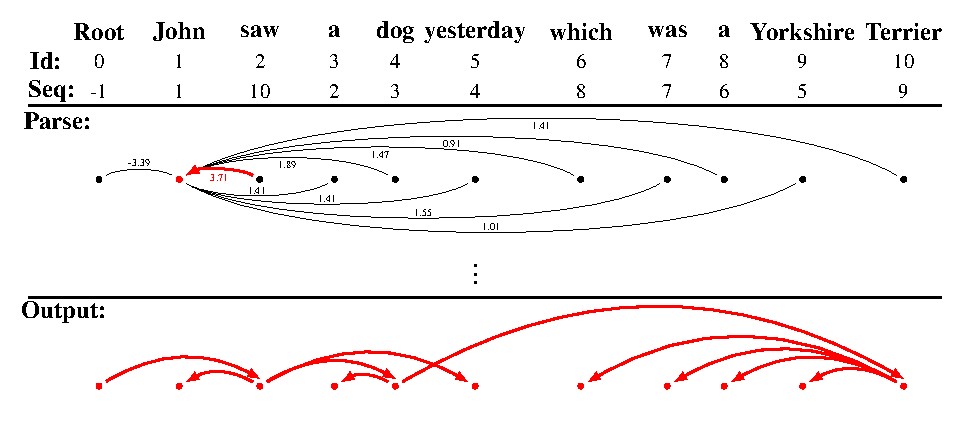
\epsfig{file=exampleparse_emnlp.eps, width=0.9\columnwidth}
\caption{Example Parse of head mapper}
%for the sentence ``\emph{John saw a dog yesterday which was a Yorkshire Terrier}". Red node is the child to be processed in every step; red arc is the final attachment from head to its dependent and dashed arc is left out to avoid circle in the parse tree.}
\label{fig:egparse}
\end{figure*}

%\KZ{The first letter of some words are missing in the figure.}
\figref{fig:egparse} shows the decoding process of the head mapper
for a non-projective example sentence~\cite{mcdonald2005non}:
``\emph{John saw a dog yesterday which was a Yorkshire Terrier}".
%\KZ{What's the original sentence? Present it first.}
%\KZ{You don't have to repeat the CoNNL format. It's not important.}
%Pseudocode shows how the head mapper works.
%Our decoder works just as the process in \figref{fig:egparse}.
%\BF{pseudocode of head mapper decoding and symbol explainations here}
A head mapper takes the lexical information of a sentence and
a permutated sequence of words in that sentence as inputs.
Suppose the sequence is: % from MaltParser:

\noindent
$John_{1}\rightarrow a_{3}\rightarrow dog_{4}\rightarrow yesterday_{5}\rightarrow Yorkshire_{9}\rightarrow a_{8}\rightarrow was_{7}\rightarrow which_{6}\rightarrow Terrier_{10}\rightarrow saw_{2}.$

The subscript stands for the position of the word in original sentence.
At step one, we look for the head of \textit{John}. At this point,
all other words are potential candidate heads. In order to measure
the probabilities of these candidate arcs, we introduce a scorer, which
is the key idea of graph-based parsers. By comparing the scores
printed on every black arc in \figref{fig:egparse},
the red arc was eventually selected, i.e. $saw$ is made the head
of $John$. The process continues for the word \textit{a}, etc.

In practice, we
%maintain a disjoint set of words processed to
ensure that
there are no cycles of nodes generated during parsing, so that the final output
is a dependency tree structure starting from
the ROOT node\footnote{A manually introduced node in dependency parsing task,
it is the root of a dependency tree.}.
We also build a parse agenda to record the existing arcs, which
provides the high order information for our scorer.
%\KZ{More details here?
%What does the parse agenda look like? How does it support high order parsing?
%Maybe use the example?}
For example, after adding arc:$saw \rightarrow John$ , all
the attachment on these two nodes will take this arc into consideration.
%For a sentence with $N$ words, the final result consists of
%($N+1$) nodes and $N$ arcs.
%\KZ{You don't need to remind people over and over again this is a combination of
%MST and Malt. You just say what you did, if it's something that MST and Malt have
%done before, be very brief about this part, and give a citation. This paper
%is about your work, not about MST or Malt.}
%Both MaltParser and MSTParser treat projective and non-projective dependency tree discriminatively. MaltParser define an extra action SWAP to generate projectivization transformation of a non-projective dependency tree \cite{nivre2009non}.
%There is a drawback of MaltParser that it cannot generate non-projective output providing projective training set, because there are no SWAP action in oracle transitions. It is sensible to look into the relation between
%possible word pairs directly. But word order limits the word pairs considered in MaltParser. MSTParser employ Chu-Liu-Edmonds algorithm to decode non-projective cases \cite{mcdonald2005non}
%and Eisner algorithm to deal with projective trees\cite{mcdonald2005online}. Though Chu-Liu-Edmonds algorithm is a solution to unify projective and non-projective cases, it declines the accuracy while applying on projective trees. Our decoder also unifies these two situations and
%searches heads globally. It directly measures the relative closeness between every possible head and current processing word and generate non-projective tree naturally.
%Head mapper tries to map head for every word stepwise according to a given process sequence of words.
%\KZ{It makes sense to include an example here to illustrate the head-mapper.}
%\subsection{Scorer and features}
%In order to simulate this process,

We introduce a linear arc scorer to measure the score of a directed arc.
The sum of all arc scores gives the final score of the whole parse tree.
%\BF{formula of arc score model}
%\[
%\text{Score}(\mathbf{y})=\displaystyle{\sum_{(i,j)\in\mathbf{y}}} \mathbf{w} \cdot \mathbf{f}(i,j)
%\]
%In this formula, $i,j$ are the indexes of an arc in parse tree $\mathbf{y}$. The inner product of arc feature vector $\mathbf{f}(i,j)$ and weight vector $\mathbf{w}$ represents score of an arc $(i,j)$. By summing up all the
%arc scores, we can get final score of the whole parse tree $\mathbf{y}$.
We currently use the typical high-dimensional binary features,
%\BF{feature template table}
including second order features \cite{mcdonald2006online}.
%\KZ{Maybe
%name some of the major features here. Don't expect the readers to
%read the MST paper.}
%As the previous statement, feature scope in graph-based parser
%is limited by decoding algorithm and several works successfully
%adapt Eisner algorithm to include high order features .
Because of the deterministic decoding in our framework,
we can make use of existing arcs to guide later head mapping.
This kind of decoder gives us the flexibility of applying any
high order features explored by previous
works~\cite{carreras2007experiments,koo2010efficient,ma2012fourth}.
%\KZ{For example?}
%\KZ{Again, you are making it sound like you only did some minor changes to MST.
%This is not the right style to write about your work. You can say we use a modified
%verion of MIRA~\cite{}, in which we did blah..}
%Based on different decoding and factoring methods, graph-based models employ different learning algorithms to induce the feature weights. Among them, variant perceptron algorithms are widely used \cite{kubler2009dependency}.

The arc scorer is trained by the iterative online
training framework MIRA (Margin Infused Relaxed Algorithm)~\cite{crammer2003ultraconservative}.
%\KZ{Give citation of MIRA itself instead of citing MST.}
\cut{
The updating constraint is defined as
\begin{align*}
&\text{min}\|\mathbf{w}^{(i+1)}-\mathbf{w}^{(i)}\|\\
&\text{s.t. } s(\boldsymbol{x}_t,\boldsymbol{y}_t)-
s(\boldsymbol{x}_t,\boldsymbol{y}')\ge L(\boldsymbol{y}_t,\boldsymbol{y}')
%\\&\forall \boldsymbol{y}'\in \text{dt}(\boldsymbol{x}_t)
\end{align*}
where $\mathbf{w}^{(i)}$ are the feature weights for the $i$-th iteration,
$\mathbf{x}_t$ and $\mathbf{y}_t$ are sentence and its gold parse tree,
respectively. $\mathbf{y}'$ is the output of our parser with $\mathbf{w}^{(i)}$ and
score margin is given out by a loss function $L$.
}
%On each update, MIRA attempts to keep the norm of the change to the parameter vector as small as possible, subject to
%correctly classifying the instance under consideration with a margin at least as large as the loss of the incorrect classifications \cite{mcdonald2005online}.
%\BF{this is the original sentence in this paper}
%Similarly, we define the loss function as the number of incorrect arcs to apply MIRA to dependency parsing and it
%is represented as following formula: \BF{Is this formula necessary ?}
%\BF{MIRA formula}
%\KZ{Don't like the following sentence.}
%From this definition, the only change we should make is replacing the exact inference decoder with our deterministic
%decoder.
In each iteration, we update the feature weights based on one sentence. The
decoder gives a greedy parse according to current feature weights.
By scoring the gold dependency tree and the current parse,
along with the number of incorrect arcs in the current parse,
MIRA keeps updating the weights until it eventually converges to an optimal scorer.
The learning algorithm typically terminates after a few iterations.
%(\figref{fig:itertest}).
%\BF{Converge graph of head mapper}
%\begin{figure}[htp]
%\centering
%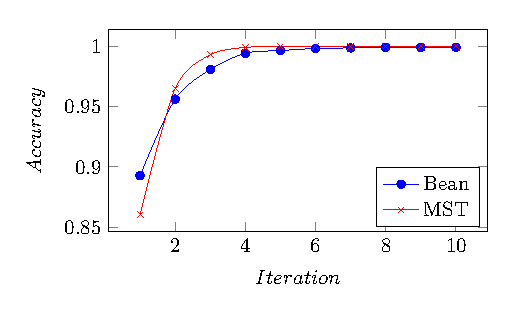
\epsfig{file=itertest.eps, width=\columnwidth}
%\caption{Accuracy curves on training set. \newline Test on first 100 sentence of WSJ senction 00.}
%\label{fig:itertest}
%\end{figure}

\subsection{Sequence Predictor}
%A sequence predictor either selects the word to process stepwise, or generates an complete word sequence.
\cut{
We developed three different sequence predictors. The first two are based on
offline training (one is a learning to rank algorithm and the other is
an action classifier used in MaltParser) from ``gold'' parsing sequences,
and produce a complete parsing sequence given a sentence.
The third sequence predictor is unsupervised and is
integrated with the decoding process, i.e. it produces the next word to
process based on the current parsing configuration.
Next we briefly discuss these three approaches.
}
%We state the rule of gold sequence in Section 2 and we can generate gold sequences with the gold dependency trees.
%Sequence predictor then learns from these gold sequences and tries to produce a sequence
%for new sentences.
%
%\subsection{Effects of Sequences}
%\KZ{Not sure what ``Sequence dependence'' means. Headings should be self-explanatory
%and clean. Consider rephrase the following paragraph. Very garbbled.}
%As we point out in section 2, getting a gold sequence from a gold dependency tree is not a one-to-one mapping.
%\BF{breadth-first traversal and malt convert sequences of example sentence}
%For example, there is a breadth-first traversal sequence of the sentence in \figref{fig:egparse},
%$which_{6}\rightarrow was_{7}\rightarrow a_{8}\rightarrow Yorkshire_{9}\rightarrow a_{3}\rightarrow Terrier_{10}\rightarrow John_{1}\rightarrow dog_{4}\rightarrow yesterday_{5}\rightarrow saw_{2}$
%, which is also a gold sequence along with the example sequence.
%\subsection{Pairwise learning to rank}
\cut{In this approach, we attempted two ways to generate gold parsing sequences.
First is a bottom-up, breadth-first traversal of the gold parse tree. This
way we are essentially processing words which are lower down in the parse
tree first, which are often less important modifiers, before moving to words
which are more central to the syntactic structure of the sentence.
The second is to take the training data from a converting function of
MaltParser, which converts a gold parse tree into a sequence of actions.
We can infer the parsing sequence of words from the sequence of actions.}

%We human beings execute a few pairwise comparisons to decide the next
%word to be processed, which is similar to preference learning problem in learning to rank.
%Sequence predicting is also a ranking process. We select next word to process by comparing it with the other words in a pairwise way.
%Viewing the task of sequence predictor in this way,
%preference learning problem in learning to rank gives a solution to predict.
\cut{
\textbf{Pairwise learning to rank }We can decompose a gold sequence into pairwise partial orders between
two words and train a binary classifer to determine the order of any two
words within a sentence. This is a popular approach in learning to rank.
However, combining pairwise orders into a complete sequence is an NP
problem~\cite{grotschel1984cutting},
we therefore use a greedy algorithm
from Schapire et al.~\shortcite{schapire1998learning} to produce such a sequence.
}
%\subsection{Action classifier in MaltParser}
The intuition of sequence predictor
is to rank words according to the ease of head word attaching.
Words that are easy to handle can be processed earlier without high order features.
To decide whether process a word immediately, we imitate the action classifier in MaltParser.
\cut{
MaltParser employs a
classifier to determine what parsing action (e.g.,
{\em shift}, {\em push}, etc.) to take at each step. The whole parsing
process defines a sequence of such actions. Although this sequence is
not exactly the word sequence used in our system, such a word sequence
can be inferred rather straightforwardly from the action sequence.

Another advantage of
the MaltParser is that it's extremely fast. Therefore, we can use MaltParser
to quickly parse through a given sentence, record the action sequence and
infer the parse sequence from it.
}
%
%Inspired by our left-to-right analysis of a sentence, we either find
%head for current word or skip this hard word and scan on. This is obviously a classification problem and
%MaltParser happen to hold the same view.\BF{cannot say so now} MaltParser add arc incrementally and provide us a potential sequence.

In fact, we can understand the action classifier in a different way that it can reflect the relative
priority between the top two words on processing stack. We translate the actiones as:
\begin{itemize}
\setlength{\itemsep}{0pt}
\setlength{\parsep}{0pt}
\setlength{\parskip}{0pt}
 \item LA - process the word on the top of stack;
 \item RA - process the second word in stack;
 \item SH - postpone the process of both the two words on top of stack.
\end{itemize}
In this way, a word sequence
can be inferred rather straightforwardly from the action sequence.

%We can decompose the predicting process into two steps:
%getting pairwise rank of every two nodes and aggregating
%these partial results into a complete process sequence.
%
%We apply LIBLINEAR\footnote{\urlstyle{same}\url{http://www.csie.ntu.edu.tw/~cjlin/liblinear/}} to training a binary classifier to get the priority of every two words. The training data are pairwise orders extracted from the gold sequence.
%The classifier can then be used to predict the relative ordering for any two words with a confidence score.
%\BF{Jia fill the details: rankSVM, Cohen, citation of preference learning}

%  \item {\bf Malt} The oracle sequence generated by converting function in MaltParser.
%  \item {\bf Random} A random permutation sequence of words for a sentence.
%  \item {\bf Increase} The left-to-right sequence, which means we process the sentence with
%  the word index increasing.
%\end{itemize}
%
%In order to test how the sequence quality influence decoding and measure different types of sequences,
%we generate four types of sequence files to test on the head mapper.
%%The train set is transformed by StanfordParser on WSJ section 2-21 and test set on WSJ section 00-01.
%Types of sequences are list below:
%Among them, the Malt sequence outperforms other types of the sequences.
%In the following, we describe a few alternative approaches to predict the sequences.
%%        \item[1] The breadth-first traversal sequence of a sentence
%        \item[2] The oracle sequence generated by converting function in MaltParser.
%        \item[3] Predicting process sequence of MaltParser stackproj algorithm.
%        \item[4] The random permutation sequence of words in a sentence.
%        \item[5] The left to right sequence, word indexes are process sequences.
%{\bf Breadth-first} The breadth-first traversal sequence of a sentence.
%
%{\bf MaltConvert} The oracle sequence generated by converting function in MaltParser.
%
%{\bf MaltPredict} Predicting process sequence of MaltParser stackproj algorithm.
%
%{\bf Random} The random permutation sequence of words in a sentence.
%
%{\bf Increase} The left to right sequence, word indexes are process sequences.
%{\small
%~\\
%
%$\bullet$ Oracle {\bf converting} sequences of MaltParser.
%
%$\bullet$ {\bf Breadth-first} traversal of a gold parse tree.
%
%$\bullet$ {\bf Predicting} process sequence of MaltParser.
%
%$\bullet$ A {\bf random} words permutation of the sentence.
%
%$\bullet$ A word sequence with {\bf increasing} index from left to right of the sentence.
%\begin{table*}[htbp]
%  \centering
%  \caption{Cross test of sequence type}
%  %\begin{threeparttable}
%    \begin{tabular}{Il|cccccIccI}
%    \whline
%    %\diagbox{Test}{Train}& Breadth-first\tnote{1} & MaltConvert\tnote{2} & MaltPredict\tnote{3} & Random\tnote{4} & Increase\tnote{5} & Average & StdDev \\
%    \diagbox{Test}{Train}& MaltConvert & Breadth-first & MaltPredict & Random & Increase & Average & StdDev \\
%    \hline
%    MaltConvert & 93.59\% & 67.32\%  & 93.29\% & 89.50\% & 83.91\% & 85.52\% & 0.109 \\
%    Breadth-first & 79.65\% & 92.36\% & 80.93\% & 86.46\% & 84.75\% & 84.83\% & 0.050 \\
%    MaltPredict & 89.30\% & 66.07\%  & 89.50\% & 87.14\% & 82.36\% & 82.87\% & 0.098 \\
%    Random & 55.41\% & 48.84\% & 56.49\% & 70.92\% & 62.77\% & 58.89\% & 0.083 \\
%    Increase & 48.89\% & 46.98\% & 48.83\% & 65.18\% & 63.36\% & 54.65\% & 0.088 \\[2pt]
%    \whline
%    \hline
%    %\midrule[3pt]
%    %     &       &       &       &       &       &     &  \\
%    Average & 73.37\% & 64.31\% & 73.81\% & 79.84\% & 75.43\%      &     & \\
%    StdDev & 0.201 & 0.183 & 0.200 & 0.110 & 0.113     &     & \\
%    \Cline{1.5pt}{1-8}
%    \end{tabular}%
%    %\begin{tablenotes}
%%        \footnotesize
%%        \item[1] The breadth-first traversal sequence of a sentence
%%        \item[2] The oracle sequence generated by converting function in MaltParser.
%%        \item[3] Predicting process sequence of MaltParser stackproj algorithm.
%%        \item[4] The random permutation sequence of words in a sentence.
%%        \item[5] The left to right sequence, word indexes are process sequences.
%%      \end{tablenotes}
%%\end{threeparttable}
%  \label{tab:crosstest}%
%\end{table*}%
%\subsection{Attempts}

%\subsection{Feature score based predictor}
%{\bf Scorer-based  }
\cut{
The intuition of sequence predictor
is to rank words according to the ease of head word attaching.
Words that are easy to handle can be processed earlier without high order features.
\cut{Words that are processed later are harder and may require high order
features. }
Since the head mapper can score every possible arc,
for each word $w$, we can compute a list of scores for all the candidate
head word of $w$. If there is a large difference in scores between the best
candidate head word and the remaining candidates for $w$,
then we can conclude the processing $w$ doesn't require high order features
and therefore can be done early.
}
%High order features are available later in the parsing process
%because many arcs have been attached by then.
%this score naturally reflects the possibility that
%a certain word can be the head of another word. We consider a word to be
%easy to deal with if
%A word is easy to deal with means that there is a head candidate much more possible than other candidates, so that it is no need to employ higher order features to find a head. In other words, greater the difference is, harder can higher order features make up for the difference.
%The intuition of sequence predictor is ranking words according to the ease
%of head word attaching. Now that the head mapper can score all possible
%head words and then choose the one with highest score, this score
%can be seen as the confidence of this arc. An arc with higher confidence
%is naturally easier to deal with.
%A word is easy to deal with means that there is a head candidate gets a higher score than the other candidates.
\cut{
As such, we maintain a matrix $M_{(n+1) \times n}$ to store the scores of
head-dependent pairs, which are initially calculated by the first order
features. When a new arc is added to the parse tree, we remove the
cells that may form a cycle with the existing arcs and update the cells
relating to this new arc using higher order features.}
%Each time we choose the word with greatest difference between its highest score and second highest score.
%After we build an arc,
 %and update sibling scores (different high order structures may require more updates).

%We will compare these three approaches in some preliminary evaluations next.
%~\\
%}
%\BF{table of cross test}

%The result of this cross test is in \tabref{tab:crosstest}. As we can
%see, training result relies much on the sequence information. Breadth-first sequence
%and MaltConvert sequence are both gold sequence of a sentence. These gold sequence models
%cannot obtain the best accuracy in other types of test sequence. Instead, the accuracy is determined
%by two factors. One is the quality of sequence, the other is matching degree between train
%sequence type and test sequence type. We can also tell from this table that we can get a
%high accuracy with a good type of sequence even on our greedy head mapper.
%
%The average accuracy and standard variance for sequence type of train file indicates the
%ability to match other types of sequence. Better sequence type gets a higher
%standard variance and a lower average accuracy. Random sequence approaches to all types in
%some sub-sequences. Increase sequence approaches to the two gold sequence because their nodes
%in the same level on gold trees mainly follow a left-to-right process rule.
%
%However, the average accuracy and standard variance for sequence type of test file shows
%the quality of a sequence type. Worse types of sequence struggles in parameter updates
%in training and better types test file can obtain a not bad result on models of worse types.
%On the contrary, worse types get bad performance on models of better types. So the accuracy
%of test file is limited by the quality of sequence type.
%%\BF{interesting conclusions: in Report201516doc, good order+ greedy head mapper->good result}
%
%Further, we print out the first-order arc heat map of same sentence.
%\BF{arc heat map}
%As we can see, different models score the arcs quite differently. Scorer relies much on the sequence and
%matched sequence pattern in train set and test set promise a high accuracy, which makes sequence predictor
%an interesting but hard task.

%
% File emnlp14-rumor\paper.tex
%
\documentclass[10pt,final,conference,letterpaper]{IEEEtran}
\usepackage{times}
\usepackage{url}
\usepackage{latexsym}
\usepackage{amsmath,algorithm,algpseudocode,caption,subcaption}
\usepackage{epsfig}
\usepackage{graphicx}
\usepackage{booktabs}
\usepackage{color}
\DeclareCaptionType{copyrightbox}
%\setlength\titlebox{6.5cm}    % Expanding the titlebox
\newcommand{\triple}[3]{$\langle$#1, #2, #3$\rangle$}
\newcommand{\pair}[2]{$\langle$#1, #2$\rangle$}
\newcommand{\figref}[1]{Figure \ref{#1}}
\newcommand{\tabref}[1]{Table \ref{#1}}
\newcommand{\secref}[1]{Section \ref{#1}}
%\newcommand{\eqref}[1]{Eq. (\ref{#1})}
\newcommand{\KZ}[1]{\textcolor{blue}{[Kenny: #1]}}
\newcommand{\WK}[1]{\textcolor{red}{[Ke: #1]}}
\newcommand{\ZY}[1]{\textcolor{red}{[Zhiyi: #1]}}

\begin{document}
\title{ExtRA: Automatic Extraction of Review Aspects 
%\Thanks{}
}

\author{
Shi Feng, Kenny Q. Zhu, Zhiyi Luo\\
%Shi Feng$~^{1}$, Kenny Q. Zhu$~^{2}$, Zhiyi Luo$~^{3}$\\
%\vspace{1.6mm}
\fontsize{10}{10}\selectfont\itshape
%Department of Computer Science \& Engineering\\
Shanghai Jiao Tong University, Shanghai, China\\
\vspace{-1cm}
%\fontsize{9}{9}\selectfont\ttfamily\upshape
%$~^{1}$sjtufs@gmail.com, $~^{2}$kzhu@cs.sjtu.edu.cn, 
%$~^{3}$jessieluo1991@gmail.com
}

%\date{\today}
\maketitle
\begin{abstract}
Summarizing users opinions about a product or
service by rating against several distinct and representative aspects
is intuitive and effective. Manual determination of aspects of a product type 
doesn't scale to large and comprehensive e-commerce or consumer review sites
and doesn't adapt to changes in interests.
This paper demonstrates a unsupervised multistage
approach for automatically discovering the best aspect words from massive
amount of textual user reviews of any type of product or service. 
Our experiments showed that the approach is efficient and achieves 
the state-of-the-art accuracies.
\end{abstract}

\section{Introduction}
\label{sec:intro}

Product reviewing is a key character that distinguishes e-commerce 
from conventional retail.
Many websites provides either qualitative or quantitative
summaries of user reviews, organized by important aspects 
of the target product or service.
One example of such \emph{aspect-based review 
summarization}~\cite{hu2004mining} for a hotel on TripAdvisor
as of June 2016 is shown in \figref{fig:tripadvisor}. 
Here, besides the short review passage written by the user, 
the user are asked to give discrete ratings (on the scale of 1-5) 
on various aspects of the hotel room, 
e.g., location and cleanness. The ratings of 
a product from individual reviews can then be aggregated into an overall
ratings of the same product by many users.

\begin{figure}[th]
\centering
\includegraphics[width=0.7\columnwidth]{figures/tripadvisor-short}
\caption{Part of a user review from TripAdvisor.}
\label{fig:tripadvisor}
\end{figure}


Aspect-based review summaries strike a nice middle ground between
detailed text reviews and an all-in-one overall score, yielding
a somewhat balanced view of a product. Such summaries
provide an effective and efficient way of comparing products in
the same category.
%have several advantages compared to the more traditional 
%style of online reviews that consists of a short passage and 
%an overall rating. 
%In aspect-based reviews, more details are provided quantitatively and 
%more directly, and the users can learn about various aspects of a product 
%without having to read the entire review passage. Another advantage of 
%aspect-based reviews is that different products within the same category 
%can be compared directly with respect to multiple aspects, 
%instead of just an overall rating. When researching on products, 
%users spend most of their time comparing different brands and models. 
%Aspect-based review summarization provides an effective and efficient way for 
%doing such comparison, saving the users both time and effort.


%At present, websites that offer aspect-based review summaries typically 
%only feature a single or a small number of product categories, e.g.,
%TripAdvisor.com only features travel related products while Cars.com reviews
%automobiles. 
Because it takes in-depth knowledge to 
characterize a product type using a few keywords that balance between
relevance and diversity, at present, these aspects are primarily hand picked
by the review site operators.
Manual selection of aspects cannot scale to large number of
product types as featured by general e-commerce platforms such as Amazon.com
and Yelp. Moreover, such aspects may change from time to time due to 
evolving user interests.
%These platforms instead turn to automatic review 
%summarization, mined from the user review texts. 

%\begin{figure}[th]
%\centering
%\includegraphics[width=0.8\columnwidth]{figures/phrases}
%\caption{Automatic review summarization for two mobile phones 
%on an e-commerce website}
%\label{fig:phrases}
%\end{figure}
%
%An example of automatic review summarization commonly seen 
%on e-commerce websites is shown in \figref{fig:phrases}. 
%There is a summary of opinion phrases for each phone model, 
%along with the frequency of each phrase mentioned in the 
%reviews. There are two major drawbacks in this form of summarization. 
%First, it is restricted to using the reviews about a specific product. 
%Therefore, summaries are incompatible across different products within 
%the same category - different models may not share the same set of 
%opinion phrases. This makes it less useful for users to compare
%different models.  Second, users' sentiment toward 
%each aspect cannot be quantified and computationally compared - 
%the difference of emotional strength between 
%``extremely good" and ``above average" is hard to capture.
% user cannot choose to express them differently.

%The aspects of a product are supposed to capture the most important features 
%and cover all the facets of the product. The products of the same category 
%share the same set of aspects, however the aspects can be very different 
%across categories. It takes both common knowledge and personal experience 
%with the product to decide which are the appropriate aspects. 
%The websites that can provide aspect-based rating system basically 
%all share a common feature, that is they each focuses on only one or 
%a small range of products. For example TripAdvisor focuses on hotels and 
%Cars.com focuese on cars. The set of aspects is what the consumers base 
%on to compare different products, thus they must be carefully chosen 
%to cover all the facest of the product. Moreoever, at the end of the day 
%the aspects is designed to serve the consumers, especially potential consumers, 
%so they need to reflect what the consumers care about the product. 
%Ideally, the aspects should be decided with user reviews taken into 
%consideration. For a small range of products, the website owner or 
%the retailer may manual designate the set of aspects, 
%however this is intractable for websites like Amazon and TaoBao, 
%which host basically all kinds of products available on the market, 
%and websites like Yelp on which users review thousands of different services. 
%
%Motivated by this observation, we are in need for methods that automatically 
%generate review summarizations. 

Our goal in this paper is to develop an unsupervised system 
for aspect word extraction from a set of user reviews about products within 
the same category.  This problem is similar to topic modeling where aspects 
can be seen as topics, but with a few differences: 
\begin{itemize}
    \item in aspect extraction, we seek to produce 
	aspect words with small mutual semantic overlap; 
    \item aspects may be expressed implicitly through personal experience; and
    \item reviews are a short piece of text, 
	  hence the topics may shift very quickly from 
          sentence to sentence.
\end{itemize}
Previous unsupervised methods for aspect extraction are 
variations of topic models, and cannot capture word semantics and thus
the implicit reference of product aspects. 
In our method we leverage the distributed 
representations of words and sentences. With distributed representations, 
the semantic similarity between two sentences can be more accurately 
calculated without relying too much on the lexical information.
Our proposed method consists 3 clustering steps and
2 ranking phases. The framework achieved state-of-the-art performance 
in end-to-end aspect extraction across multiple domains.

%In \secref{sec:method} we introduce our method step-by-step.
%In \secref{sec:experiments} 
%we evaluate our method on user reviews from multiple domains and demonstrate 
%the effectiveness of our model against other approaches 
%and show how the aspects extracted can be used
%to construct a complete review summarization. 
%In \secref{sec:related}, we discussed
%and compare our work with previous research on aspect-based review 
%summarization.

\section{The System}
\label{sec:method}

The review aspect extraction problem aims to infer $K$ noun 
words from user reviews about the same product type.
Each word represents a distinct aspect or feature of the product type. 
%Here $K$ is an constant parameter for the problem. 
%In unsupervised models for aspect extraction, 
%the set of reviews and the number of aspects are the only inputs.
%Note that in this definition we don't use cross-domain information, 
%that is, for one product type we only use the reviews of that domain.
%This allows us to apply the model to any domain with ease.
%\begin{figure}[th]
%\centering
%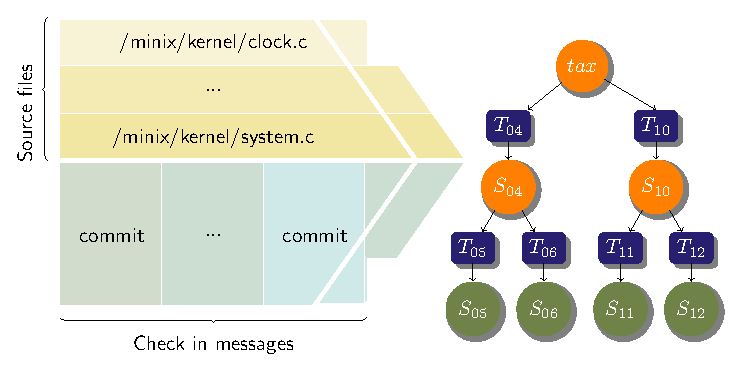
\includegraphics[width=0.9\columnwidth]{figures/framework}
%\caption{Our framework.}
%\label{fig:framework}
%\end{figure}
%
Our system framework consists of 5 steps.
%
%\begin{itemize}
%    \item \textbf{Sentence Clustering}
%
%        We convert each sentence in the reviews into a vector representation 
%        and cluster them in to $N$ clusters of semantically similar sentences.
%
%    \item \textbf{Noise Isolation}
%
%        %As aspects appear as topics in the reviews, 
%        %we use a topic model to infer the potential aspects.
%        To isolate the noises that exist in the sentence cluster,
%	for each sentence cluster we further generate $M$ 
%	topics, resulting in $N\times M$ different word distributions in total.
%
%    \item \textbf{Aspect Inference}
%        
%        We treat each word distribution as a vector and cluster the topics 
%	into $C$ clusters which are the potential aspects. 
%	Here $C$ is purposely set to be larger than $K$. The extra
%	$C-K$ clusters models the redundant aspects.
%        Each cluster contains $N\times M / C$ word distributions, or vectors.
%        We take the mean of these vectors to form $C$ aspect clusters,
%        each being a set of words and their corresponding weights.
%
%    \item \textbf{Cluster Ranking}
%
%        We define a score for the quality of each aspect cluster,
%        and the clusters are ranked by this score.
%
%    \item \textbf{Word Ranking}
%
%        We use WordNet to calculate the semantic distances between the words 
%	in each cluster and adjust the ranking based on the 
%	both the distances and the weights of the words. The top words in each
%	cluster are candidates of the aspect words.
%\end{itemize}
%
%In the following we will explain the motivation and the details of each of
%the five steps. 
%
\subsection{Sentence Clustering}

%One important feature of user reviews is that many topics are 
%compressed into a short paragraph, where each topic corresponds to 
%a potential aspect of the product. 
%A typical hotel review extracted from \figref{fig:tripadvisor} 
%is shown as follows:
%
%\begin{quote}
%Pool is small and only 4 ft but refreshing. Hot tub also there. Staff were super friendly each day. Room was nothing special but clean and comfy. Lots of restaurants and bars nearby. Breakfast was great and despite being a busy weekend there was always a big selection available.
%\end{quote}
%
%In user reviews, topics can shift very quickly.
%Sentences that are close to each other may refer to 
%completely different aspects about the product. Also,
%sentences about the same aspect may not appear in the review consecutively. 
%The existence of such fine-grained semantic shifts in user reviews 
%makes it difficult to apply the the bag-of-word abstraction 
%of normal topic model on reviews.
%Therefore we propose to work on the sentence level instead 
%of the document level, and it would be helpful if we can divide the 
%reviews into topic-oriented segments.
%
%Driven by this observation, in our method the first step is 
%sentence clustering.  For this purpose, 
We represent each sentence in a high-dimensional vector space,
%Instead of using simplistic methods like bag-of-word vector, 
%we leverage a recent development of neural network in natural 
%language processing, the distributed representation.
%In a distributed representation, words and sentences are 
%converted into real-valued vectors.
%The distance of the vectors in the vector space will capture the 
%semantic similarity of the words or sentences.
%In this work we attempt two models, 
using either LSTM (a variant of RNN) or paragraph vector (PV) \cite{le2014distributed}.
%
%\paragraph{Recurrent Neural Network}
%To use RNN for obtaining sentence vectors, 
%we train a neural language model on the review sentences. 
%After the perplexity converges, we use the trained network to 
%process each sentence of the dataset and take the last hidden vector as 
%the vector representation of the sentence. In our method we use a 
%variation of RNN, long-short term memory (LSTM)~\cite{hochreiter1997long} 
%which is reported to have better performance at 
%modeling long sentences \cite{jozefowicz2015empirical}.
%
%\paragraph{Paragraph Vector}
%PV is a simple but powerful extension to Word2vec \cite{mikolov2013distributed} with two components, 
%distributed memory (PV-DM) and distributed bag-of-word (PV-DBOW). 
%The first one is similar to skip-gram in Word2vec and 
%the second is similar to CBOW \cite{mikolov2013distributed}.
%An important advantage of paragraph vector models is that they require 
%no labeled data. Also, it doesn't require human experts to assign weights 
%for words in a paragraph based on linguistic knowledge. 
%The learned vector representations inherit an important property of Word2vec, 
%that is the semantics similarity. Also the final paragraph vector captures the 
%word order information with the part learned from PV-DBOW with the n-gram model.
An advantage of paragraph vector over RNNs is that it can 
leverage trained word vectors, thus requires a smaller training data set. 
%The word vectors can be trained on 
%a much larger corpus so they capture the semantics relationships more 
%accurately.  Consequently, the paragraph vectors can be trained on 
%a relatively small dataset. 
%The performance of paragraph vectors can also be boosted by using pre-trained 
%word vectors that are trained on a larger dataset \cite{mikolov2013linguistic}. 
%%However, previous research show that it is more suitable 
%%to train the word vectors simultaneously for RNNs, 
%%so RNNs cannot leverage the word vectors learned from a larger dataset. 
%Also, the paragraph vector models are simple and 
%don't require the storage of a lot of information. In contrast, for RNN we 
%need to store every state during the forward pass for back-propagation, 
%which is very memory consuming.
%\paragraph{Clustering Sentence Vectors}
We run k-means clustering on the sentence vectors and generate 
$N$ sentence clusters. We then collect the sentences from the same review 
that are clustered together to form smaller fragments of reviews. 
Each original review is divided into several smaller review fragments, 
each belonging to one of the $N$ clusters. As a result, we obtain $N$ 
clusters of review fragments. 

\subsection{Noise Isolation}
There exists noises and overlaps in the clusters formed above.
%The first step, sentence clustering, we might include noise and the sentences 
%within a cluster might not all be about the same aspect. 
%The reason is due to the common occurrences of sentences such as the following
%in the reviews (taken from TripAdvisor):
%
%\begin{quote}
%The room was clean, the staff were friendly, and I would say the price is very reasonable given the proximity to business and leisure destinations around downtown.
%\end{quote}
%
%\begin{quote}
%There is a restaurant just 5 min walk away with nice italian food, pizza was great.
%\end{quote}
%
%In the first sentence multiple aspects are mentioned; in the second sentence, the only aspect is location however lexically it seems to be talking about food.
%With these complicated structures within, 
%it is difficult for RNN or PV to correctly determine the aspects 
%in these sentences. The result is overlaps between clusters about 
%different aspects and noises within each cluster.
%To isolate the noises and resolve such overlap, 
We fix that by applying LDA topic modeling within each sentence cluster, 
treating each review fragment as a document, and generating $M$ smaller topics. 
This will give us in total $N\times M$ topics, or, word distributions. 
%\tabref{table:overlap} shows an example of topics inferred from three
%sentence clusters from hotel reviews and illustrates the overlap problem.
%In this example, five topics were extracted from each sentence cluster, 
%and each row is one topic. It can be seen that the aspects for the 
%three clusters should be {\em room}, {\em location} and {\em price} 
%respectively.
%However, topics shown in boldface font obviously belong to 
%other clusters.  Especially, the last topic of the third cluster 
%appears to be an overlap of more than two clusters.
%The noise isolation step effectively separates the noise topics from other
%topics semantically corehent within a sentence cluster.
%
%\begin{table}[th]
%\centering
%\caption{Topics extracted from three sentence clusters of hotel review.}
%\label{table:overlap}
%\begin{tabular}{|c|l|}
%\hline
%& room bed bedroom size floor \\
%Sentence
%& bedroom room wall size decor \\
%cluster 1
%& room bathroom shower water towel \\
%& room suite size view floor \\
%& room shower area kitchen bed \\\hline
%
%& station minute tube location bus \\
%Sentence
%& location price night place rate\\
%cluster 2
%& location square station street subway\\
%& distance bus subway downtown shopping\\
%& \textbf{restaurant} \textbf{city} \textbf{food} \textbf{buffet} \textbf{place} \\\hline
%
%& price rate service money star\\
%Sentence
%& \textbf{location} \textbf{city} \textbf{star} \textbf{time} \textbf{rate} \\
%cluster 3
%& price service night money city\\
%& price location place night city\\
%& \textbf{location} \textbf{service} \textbf{food} \textbf{price} \textbf{restaurant} \\\hline
%\end{tabular}
%\end{table}


\subsection{Aspect Inference}
\label{sec:topic_clustering}
Each topic is a word distribution, represented by a vector. 
We obtain  more compact representations of those topics by using PCA to 
reduce the topic vectors to 100-dimension.
%We use PCA to reduce the topics vectors to 100-dimension by  
%selecting the 100 words that best distinguish different topics.
Then we perform k-means clustering on the $N\times M$ topics vectors to 
generate $C$ clusters, each containing $(N\times M)/C$ topics.
These are called {\em aspect clusters}.
We set $C$ to be slightly larger than the desired number of product 
aspects $K$, so that the noisy topics can be clustered together and 
later discarded. 
%In an experiment we will evaluate the influence of this redundant clusters on 
%the quality of the final aspects.
%
%\begin{table}[th]
%\caption{Aspect clusters extracted from hotel reviews.
%Each row shows the candidate words of an aspect, sorted by the weight of each word.}
%\label{table:step3}
%\centering
%\begin{tabular}{|l|} \hline
%breakfast, meal, food, tasty, dinner, morning, coffee, tea \\\hline
%room, night, time, bed, day, bathroom, staff, area, place \\\hline
%staff, desk, service, friendly, reception, concierge, helpful \\\hline
%close, city, location, place, central, station, bus, street\\\hline
%bed, shower, spacious, room, size, bathroom, bedroom, floor \\\hline
%price, room, check, night, money, city, location, star, service \\\hline
%location, price, room, night, place, rate, money, time, city  \\\hline
%\end{tabular}
%\end{table}
%
%Finally, for each cluster we take the mean of the $(N\times M)/C$ 
%topics and normalize it
%for the word distribution of that cluster.
%Some example aspect clusters extracted from hotel reviews are 
%shown in \tabref{table:step3}.

\subsection{Cluster Ranking}

We rank the clusters by how ``distinct'' each cluster is from other clusters. 
If a cluster is similar to other clusters, it is considered redundant and of
low quality. We discard $C-K$ least distinct clusters.


%For the $i$th cluster $C_i$ ($i\in [1, C]$), 
%the distinctiveness score $S(i)$ is defined by:
%
%\begin{align}
%S(i) &= \sum_{w\in C_i} S_i(w) \nonumber\\ 
%     &= \sum_{w\in C_i} \log\left(\frac{f_i(w)}{\sum_{j\neq i} f_j(w)}\right)\nonumber \\
%     &= \sum_{w\in C_i}\left[\log f_i(w) - \log\sum_{j\neq c} f_j(a)\right]
%\end{align}
%
%\begin{table}[t]
%\caption{Aspect clusters ranked by distinctiveness score.
%Potential aspect words are boldfaced.}
%\label{table:clustersranked}
%\centering
%\begin{tabular}{|l|} \hline
%\textbf{staff}, desk, \textbf{service}, friendly, reception, concierge, helpful \\\hline
%breakfast, meal, \textbf{food}, tasty, dinner, morning, coffee, tea \\\hline
%\textbf{price}, room, check, night, money, city, location, star, service \\\hline
%bed, shower, spacious, \textbf{room}, size, bathroom, bedroom, floor \\\hline
%close, city, \textbf{location}, place, central, station, bus, street \\\hline
%\textcolor{red}{room, night, time, bed, day, bathroom, staff, area, place} \\\hline
%\textcolor{red}{location, price, room, night, place, rate, money, time, city} \\\hline
%\end{tabular}
%\end{table}
%
\subsection{Word Ranking}
\label{sec:word_ranking}

We rank the words in each cluster 
by considering two factors (similar to TF-IDF): 
the representativeness of the word to the host
cluster; the number of times the word appears in other clusters. 
The most representative word in each cluster
is assumed to be the closest to the centroid of the word cluster.
The distance between two words is the inverse of 
cosine similarity between the word2vec
vectors of the two words.
Then we process the clusters in the order of 
the cluster ranking given in the last step.
When we calculate the score for word $x$ cluster $C_i$,
we also consider the scores of word $x$ in clusters $C_1$ to $C_{i-1}$, 
where the scores have already been calculated. 
We prevent the duplicate aspect words by subtracting the scores 
of $C_1$ to $C_{i-1}$, from the score of $C_i$.
%The score of word $x$ in the $i$th cluster $C_i$ is thus defined by:
%
%\begin{equation}
%s_i(x) = u_i(x) \sum_{y\in C_i}\hat{x}\cdot \hat{y} - \sum_{j=1}^{i-1}s_j(x),
%\label{eq:wordscore}
%\end{equation}
%where $\hat{x}$ is the vector representation of x; $u_i(x)$ is the weight of $x$ in cluster $C_i$.
The words in each cluster is thus ranked by this final score.

\section{Evaluation}
\label{sec:experiments}

We evaluated our framework
against a number of baselines including the state-of-the-art approaches.
%in the end-to-end aspect extraction task.
Our dataset is reviews for 15 categories of product or service crawled from
e-commerce sites such as Amazon.com and Yelp. 
%The review content is plain English text and we do not use any labels 
%for training our model. We use human labels for evaluation. 
%The product categories, their sources and the sizes of the review datasets
%are summarized in \tabref{table:dataset}
%
%\begin{table}[th]
%\centering
%\caption{Dataset summary.} 
%\label{table:dataset}
%\begin{tabular}{|c|c|r|r|}
%\hline
%Product type & Source & No. of Reviews & No. of Words \\ \hline \hline
%hotel        & TripAdvisor & 27145   & 210 \\\hline
%mobile phone & Amazon & 3716    & 136 \\\hline
%mp3 player   & Amazon & 2745    & 128 \\\hline
%laptop       & Amazon & 5471    & 97  \\\hline
%tv           & Amazon & 1237    & 102 \\\hline
%shoes        & Amazon &1748    & 82  \\\hline
%headphone    & Amazon & 1647    & 122 \\\hline
%gps          & Amazon & 1726    & 72  \\\hline
%transportation & Yelp & 3077  & 131 \\\hline
%restaurant   & Yelp & 4016    & 176 \\\hline
%gym          & Yelp & 2481    & 230 \\\hline
%shopping     & Yelp & 2718    & 123 \\\hline
%car dealer   & Yelp & 2839    & 190 \\\hline 
%movie        & Pang et al. \cite{pang2002thumbs} & 3000    & 194 \\\hline
%car          & Cars.com & 1074    & 147 \\\hline
%\end{tabular}
%\end{table}
%
%
%For evaluation, we ask 5 college students proficient with English 
%to annotate ground truth
%aspect words for each product category. For each category, 
%we ask them to provide 5 different words that cover the most important 
%aspects of the corresponding product or service. The labels provided by the
%5 annotators are aggregated together without removing duplicated words, 
%so we have 25 words in total. 
%When evaluating the models, 
%we compare the 5 aspect words generated by the models with those provided 
%by the annotators. 
%We calculate the portion of words among the 25 labels that 
%are correctly generated by the model as the accuracy of the model.
%The ground-truth labels for two product categories are shown 
%in \tabref{table:labels}.
%
%
%\begin{table}[th]
%\centering
%\caption{Labels for hotel and shopping. Each row is provided by one annotator.}
%\label{table:labels}
%\begin{tabular}{|c|l|}
%\hline
%\multirow{5}{*}{hotel}
%& room price location service utility \\
%& room service price food location  \\
%& sleep service room price location  \\
%& location price bedroom bath staff  \\
%& room price bath staff location  \\\hline
%
%\multirow{5}{*}{shopping}
%& location product service price environment \\
%& product price service location ambience \\
%& price food location size facility \\
%& sales location food service environment \\
%& price location service facility food \\\hline
%\end{tabular}
%\end{table}
%
%\subsubsection{Parameter Tuning}
We conduct a few experiments to determine the following
parameter settings: $N=10$, $M=10$, $C=K+2$, i.e. at most two extra clusters.

We compare 5 models in our experiments, 
LDA as a simple baseline, 
D-PLDA \cite{moghaddam2012design} as a representative for joint 
aspect-sentiment models, MG-LDA \cite{titov2008modeling} as 
a representative for aspect extraction topic model,
and two variations of our model LSTM and PV. 
We run the 5 models on the review data of each product type separately. 
For the main experiment, the number of aspects is fixed to 5.

%\begin{figure*}[th]
%\centering
%\includegraphics[width=1.9\columnwidth]{figures/results}
%\caption{Accuracies from different models.}
%\label{fig:results}
%\end{figure*}
%In the end-to-end evaluation, we compare the performance of our models on aspect extraction with three other models as mentioned above. The results are shown in \figref{fig:results}. 
By the accuracy, our two models out-performed all other models in 13 out of 15 
categories. The PV model performs better LSTM, 
which is consistent to our earlier analysis. \tabref{table:hotel_aspect_words}
shows the 5 aspect words by each model for hotel reviews.

\begin{table}[th]
\centering
\small
\caption{Top aspect words for hotels by different models}
\label{table:hotel_aspect_words}
\begin{tabular}{|l|l|} \hline
Ours(PV) & staff, food, price, room, location \\ \hline
Ours(LSTM) & service, location, time, food, bed\\ \hline
MG-LDA & shower, time, food, room, price\\ \hline
DP-LDA & service, station, check, coffee, bed \\ \hline
LDA & stay, location, room, staff, room \\ \hline
\end{tabular}
\end{table}
 
\section{Demo Scenarios}
We present a web demo which depicts the following scenario.
The user logs on and selects
a product type, e.g. ``cell phones'', from a predefined set of categories,  
and sets the number of aspects $K$. 
Then the user clicks the ``generate" button to extract $K$ aspect words for the selected product type.
Upon this, the system computes the review summaries of all cell phones. 
%Upon this, the system shows the $K$ precomputed aspect words for that
%product type, computed from the many user reviews about ``cell phones''. 
%Then the user clicks a button to ``generate review summaries'', which presents
%the review summaries of all cell phones in
%the system. 
Each summary contains the aspects and their scores, computed from the sum of
sentiment scores (1, 0 or -1) against each aspect using LSTM trained on
Stanford Sentiment Treebank~\cite{socher2013recursive}. 
The user may filter out some of the 
results by using the search box (see \figref{fig:summary1}). 
If the user wishes to understand why a product receives a score for a 
certain aspect, they can click on the ``xxx customer reviews'' link
and be directed to the original review snippets with the aspect words and 
sentiment words highlighted. The review snippets by can further grouped by
aspects by clicking on the tabs (see \figref{fig:summary2}). 

\begin{figure}[th]
\includegraphics[width=\columnwidth]{figures/demo1.png}
\caption{Automatically generated 6 aspects for cell phones}
\label{fig:summary1}
\end{figure}

\begin{figure}[th]
\includegraphics[width=\columnwidth]{figures/demo21.png}
\caption{Review snippets displayed by the aspects}
\label{fig:summary2}
\end{figure}


%The second and a minor scenario enables the user to examine the dynamic change
%in aspect words over time for each product type. The system shows a time line,
%annotated with different sets of aspect words, by configurable time periods,
%e.g., every month, 6 months or a year.  
 
\bibliographystyle{IEEEtran}
\bibliography{master}
\end{document}

\section{Conclusion}
We implement a novel sequence-based dependency parsing
framework which takes advantage of high order features 
in parsing history. 
%We can also adapt beam search to this framework so as to
%relax the strictly greedy nature. Vine pruning\cite{rush2012vine} could
%be incorporated to speed up the parsing.
More importantly, we discovered that the parsing accuracy is very sensitive to
the quality of parsing sequence. Future work can be focused on
developing better sequence predictors that outperform Malt action classifier.
Furthermore, we use two sets of features for sequence predictor and
head mapper right now. A unified set of features between these two components
are worth exploring.
%Besides, better sequence predicting method and unified feature
%representation of two components are worth exploring.
%
%Though we currently get a not bad result,
%the sequence predictor still needs more exploration.
%According to our experiment, slightly changes
%on the sequence can lead to a fatal decline on accuracy. Ensuring the match degree of training sequence and testing
%sequence demands a high quality of sequence predictor.
%
%Further, the features in our current implementation are not expanded and well tuned yet  and we are free to define high order features to make use of parsing history. Our framework is flexible to merge other technics to enhance the performance. Introducing beam could make up for our greedy decoder and improve our accuracy. Vine pruning\cite{rush2012vine} could speed up parsing process. Besides, better sequence predicting method and unified feature representation of two components are worth exploring.




\bibliographystyle{acl}
\bibliography{parser}

\end{document}
